\documentclass[9pt,twocolumn]{article}
%\usepackage[font=small,margin=1in]{caption}
%\documentclass[11pt]{article}
\usepackage[font=small]{caption}
\usepackage[numbers]{natbib}
\usepackage{amsthm,amsmath,amssymb}
\usepackage{multirow}
\usepackage[pdftex]{graphicx}
\usepackage{subfigure}
\usepackage{makecell}
\usepackage{booktabs}
\usepackage{array}
\usepackage{fullpage}
\usepackage{algorithm}
\usepackage{algpseudocode}
\usepackage{algorithmicx}
\usepackage{framed}
\usepackage{bm}
\usepackage{mathtools}
\usepackage{wrapfig}
\usepackage{lipsum}
\usepackage{mathrsfs}
\usepackage{dsfont}
\usepackage[colorlinks=true,
            linkcolor=blue,
            urlcolor=black,
            citecolor=blue]{hyperref}
 %IF you want section & subsection heading to be in line
\usepackage{titlesec}
\titleformat{\section}[runin]
  {\normalfont\large\bfseries}{\thesection}{0.4em}{}
\titleformat{\subsection}[runin]
  {\normalfont\normalsize\bfseries}{\thesubsection}{0.4em}{}

%%%%%%%%%%%%%%%%%%%%%%%%%%%%%%%%%%%%%%%%%%%%%%%%%%%%%%%%%%%%%%%%%%%%%
\setcounter{page}{1} % start with first page

\begin{document} % goes here
\sloppy
\title{\Large{\textbf{
Measuring the effect of COVID-19 lockdowns on air quality and\\
the impact on child health using machine learning
}}}

\author{
Jonathan Baron\thanks{Department of Psychology, University of
  Pennsylvania. Email: baron@upenn.edu.}\;\,\thanks{Some other address.}
\and 
  Some O. Person\thanks{Yet another place.} 
\and
  Y. Another Author\footnotemark[2] % indicates same as 2nd thanks
}

\date{} % leave empty
\maketitle
%\thispagestyle{firstpage}

\begin{abstract}

blah\smallskip
\noindent

Keywords: journal, template, latex

\end{abstract}

%{\renewcommand{\thefootnote}{}
%\footnotetext{ % note blank lines above and below acknowledgment
%
%
%Copyright: \copyright\ 2021.
%The authors license this article under the terms of the
%\href{http://creativecommons.org/licenses/by/3.0/}{Creative Commons
%  Attribution 3.0 License.}
%}}
\section{Introduction}\label{sec:intro}
UNICEF and Solve for Good have partnered together to analyze various aspects of changes in air pollution — especially related to COVID-19 and with the long-term goal to build a platform for air pollution monitoring with a strong emphasis on UNICEF’s operations, with focus on
\begin{itemize}
    \item Developing a model to measure children’s exposure to air pollutant PM2.5, which exceeds the WHO Standard in the present COVID Scenario.
    \item Understanding the air quality level around the globe with the target of attaining a fine-grained estimation from the combination of Ground value measurement from openly available ground sensor measurements and Remote Sensing
    \item Enabling Citizen Scientists to delve deeper and get involved in Air Quality Measurement globally.
\end{itemize} 
%
Specifically, we aim to (a) model the impact of COVID19 lockdowns on air quality and (b) test whether this has led to an improvement in children’s health. Following the footsteps of existing works like \citet{Borneman,Mahato}, we hypothesize to find evidence of the positive effects of air quality resulting from the large-scale modal shift to low emissions vehicles post lockdown develop an exploratory visualization platform for local program managers. The platform will provide functions to manage, analyze, and visualize changes in air pollution data at different locations preferably, in countries and cities where UNICEF operates with interests in air pollution monitoring for children’s health.

Globally, 93\% of children live in environments where air pollution levels exceed WHO guidelines. There is a strong link between human health and exposure to high levels of air pollution. Long-term exposure to fine particulate matter with a diameter less than 2.5$\mu$m (PM2.5) are estimated to cause ~8 million excess deaths annually. Simultaneously, nitrogen dioxide (NO$_2$) results in 4 million new pediatric asthma cases annually \cite{Venter}. The impact of air pollution is felt more acutely by the young, with one in every four deaths of children under 5 years is directly or indirectly related to environmental risks \cite{who}.

However, the child population’s distribution does not correspond well to the global distribution of air quality sensors. Illustrating these distributions are panel (a) of Figure~\ref{fig:maps} showing the locations of air quality sensors and panel (b) the global concentration of child populations. Therefore using only the locations of ground-source air quality sensors to infer the effects of exposure to high levels of air pollution on global child populations is difficult, particularly in high populous locations such as Western Africa and the Great Rift Valley.

\begin{figure*}
    \centering
    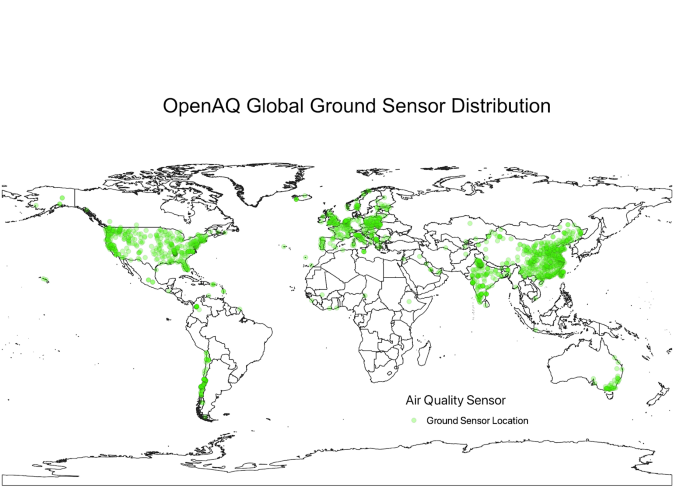
\includegraphics[width=.49\textwidth]{sensormap.png}
    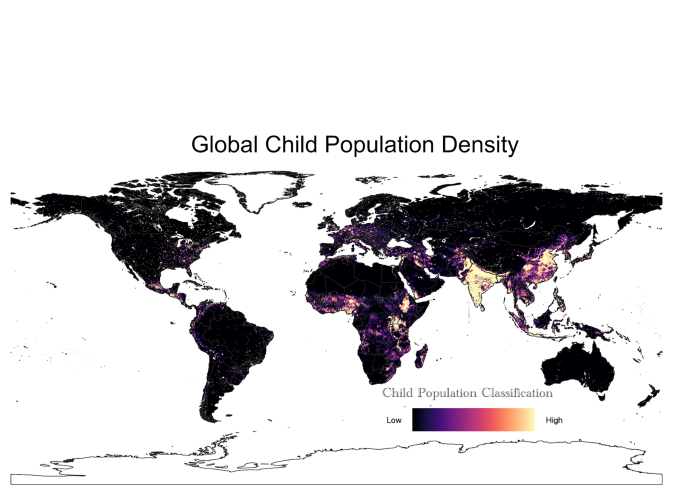
\includegraphics[width=.49\textwidth]{childmap.png}
    \caption{Global distribution of (a) air quality sensors, and (b) Child Population, data source: Silent Suffocation in Africa, UNICEF-2019.}
    \label{fig:maps}
\end{figure*}

During the Covid-19 lockdowns, fossil fuel consumption has decreased due to lower mobility levels in general, as well as a shift to low-emission modes of transport (such as walking and cycling). This prevents previous models that measure the global distribution of air pollution inaccurate, as they are unable to represent the current changes in air pollution levels due to COVID19 lockdown events \cite{stateof}.

The decreased concentration of harmful emissions resulting from this has the potential to significantly improve cardiovascular health for children, who are more vulnerable to the impact of air pollution \cite{Rees}. At UNICEF and Solve for Good, we wanted to question the children’s health to the global air quality emissions data UNICEF collected during the lockdown to identify if there is a significant improvement in child health with a mass transition to low carbon energy sources for industry and vehicles.
We take a 3 step approach to our analysis.

\begin{enumerate}
    \item We develop a large-scale model aimed at providing air quality predictions across geographic regions using widely available data sources,
    \item Develop a geospatial visualization platform for the exploration of results,
    \item Fine-tune results of the large-scale model using location-specific heterogeneous data sources for more accurate local-level predictions, and correlate results with child health indicators.
\end{enumerate}

%We focus on the first two steps in this article series. The first article discusses the importance of air quality monitoring, the available data sources, data setup, and some exploratory results in the current context. In the second article, we shall discuss the details and results pertaining to the global level model. The third article will be aimed at visualization and discussion of results, as well as pointers towards future work on local models and incorporating child health data.
\section{Data}\label{sec:data}

\subsection{Data sources}
We collect air pollution levels using 1600 air quality stations measuring ground-level PM2.5 concentrations from January 2019 to September 2020 from OpenAQ\footnote{\url{https://openaq.org}} as our target variable. To predict PM2.5 concentrations, we extract weekly averaged time-series values for AOD, NO$_2$, Land Use, and Precipitation satellite data from Google Earth Engine. To extract data from the Google Earth Engine\footnote{\url{https://earthengine.google.com}}, we import data from 1st January 2019 to 11th September 2020 from the following satellites:
%
\begin{itemize}
    \item Sentinel-5P NRTI NO$_2$: Near Real-Time Nitrogen Dioxide (NO$_2$),
    \item MCD19A2.006: Terra \& Aqua MAIAC Land Aerosol Optical Depth Daily 1km (AOD),
    \item GPWv411: Population Density Gridded Population of the World (Population Density),
    \item GSMaP Operational: Global Satellite Mapping of Precipitation (Precipitation).
\end{itemize}

\subsection{Data Processing}
The satellites collect data at different temporal and spatial granularities (Table~\ref{tab:datatable}). To standardize the satellite data, we aggregate the satellite data by weekly average (Figure~\ref{fig:2step}). To generate these statistics, we generated a VRT driver (a format driver for GDAL that allows a virtual GDAL dataset to be composed from the other GDAL datasets) to process the data faster.

\begin{table*}[t]
\centering
\begin{tabular}{l|llll}
\toprule
\parbox[t]{2cm}{{\bf Data\\name}} &
\parbox[t]{2cm}{{\bf Data\\type}} &
\parbox[t]{3cm}{{\bf Spatial\\resolution}} &
\parbox[t]{2cm}{{\bf Temporal\\resolution}} &
\parbox[t]{5cm}{{\bf Description}}\\\midrule
\parbox[t]{2cm}{PM2.5} &
\parbox[t]{2cm}{Ground\\Sensor} &
\parbox[t]{3cm}{Point location\\(latitude/longitude)} &
\parbox[t]{2cm}{Hourly} &
\parbox[t]{5cm}{Weekly averaged PM2.5 collected by ground station, source: OpenAQ}\\\midrule
\parbox[t]{2cm}{Oxford COVID19 Data} &
\parbox[t]{2cm}{Tabular} &
\parbox[t]{3cm}{National\\(192 countries)} &
\parbox[t]{2cm}{Daily} &
\parbox[t]{5cm}{Lockdown information}\\\midrule
\parbox[t]{2cm}{Precipitation} &
\parbox[t]{2cm}{Raster} &
\parbox[t]{3cm}{0.1 arc degrees} &
\parbox[t]{2cm}{Daily} &
\parbox[t]{5cm}{Snapshot of hourly precipitation rate, source: GSMaP Operational}\\\midrule
\parbox[t]{2cm}{AOD} &
\parbox[t]{2cm}{Raster} &
\parbox[t]{3cm}{1000 meters} &
\parbox[t]{2cm}{Daily} &
\parbox[t]{5cm}{Blue band (0.47 $\mu$m) aerosol optical depth over land, source: MCD19A2.006}\\\midrule
\parbox[t]{2cm}{NO$_2$} &
\parbox[t]{2cm}{Raster} &
\parbox[t]{3cm}{0.01 arc degrees} &
\parbox[t]{2cm}{Daily} &
\parbox[t]{5cm}{Total vertical column of NO$_2$ = ratio of NO$_2$ slant column density and total air mass factor, source: Sentinel-5P NRTI NO$_2$}\\\midrule
\parbox[t]{2cm}{Population Density} &
\parbox[t]{2cm}{Raster} &
\parbox[t]{3cm}{30 arc seconds} &
\parbox[t]{2cm}{Daily} &
\parbox[t]{5cm}{The estimated number of persons per square kilometer, source: GPWv411}\\\midrule
\parbox[t]{2cm}{Average\\Pop. Den.} &
\parbox[t]{2cm}{Tabular} &
\parbox[t]{3cm}{National} &
\parbox[t]{2cm}{Yearly} &
\parbox[t]{5cm}{}\\\midrule
\parbox[t]{2cm}{Sensor\\Latitude} &
\parbox[t]{2cm}{Tabular} &
\parbox[t]{3cm}{10m} &
\parbox[t]{2cm}{N/A} &
\parbox[t]{5cm}{}\\\midrule
\parbox[t]{2cm}{Sensor\\Longitude} &
\parbox[t]{2cm}{Tabular} &
\parbox[t]{3cm}{10m} &
\parbox[t]{2cm}{N/A} &
\parbox[t]{5cm}{}\\\bottomrule
    \end{tabular}
    \caption{Details on the datasets used.}
    \label{tab:datatable}
\end{table*}

\begin{figure}[t]
    \centering
    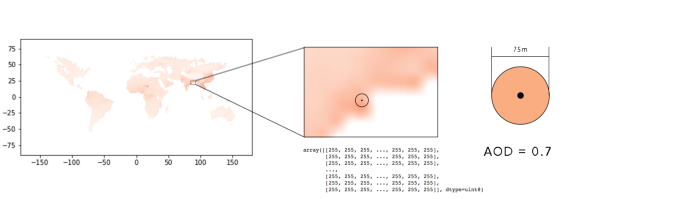
\includegraphics[width=\linewidth]{2step1.png}
    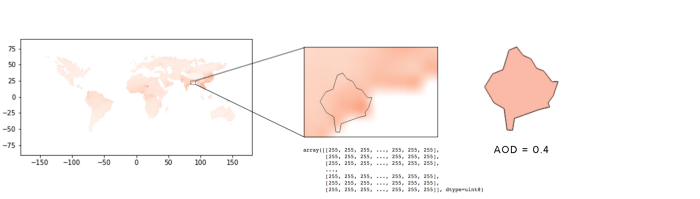
\includegraphics[width=\linewidth]{2step2.png}
    \caption{Panel (a) illustrates the ``local” extraction of AOD from a 75m buffer around a point. Panel (b) illustrates the “city-level” extraction of AOD for each city globally. AOD = Aerosol Optical Depth is a well-known proxy for PM2.5 \cite{Kumar}.
}
    \label{fig:2step}
\end{figure}

Using the VRT file, we extracted weekly averaged data for each of the cities using their geometric shapes. We utilize GADM Shapefiles for this purpose to mask the images and obtain weekly satellite variable averages for city shapes. We extracted weekly averaged data at two different geographic levels, at the local and city-wide levels. At the local level, we extract weekly averaged satellite data values using a local mask defined as a 75m buffer around a ground sensor location. We extract city-wide weekly averaged satellite data values using corresponding city masks from GADM city polygons\footnote{\url{https://gadm.org/data.html}}. In addition to incorporating satellite data as features in the machine learning model, we include several secondary data sources, such as the Covid-19 ``Stringency index" across different spatial and temporal resolutions. See Table 1 for details on the data sources.

Furthermore, we preprocess the PM2.5 station data to ensure we had a reliable training dataset. To do so, we removed PM2.5 values above and equal to 3000 and values below 0. We resampled the PM2.5 values on a weekly basis (Monday Start Day) and use the mean. Using the 75m buffer and the city-wide polygons, we averaged the weekly PM2.5 value for a 75m radius around the sensor’s location point. We averaged the weekly PM2.5 value for the city extent if the point is within the city in GADM. Our final preprocessing step was to aggregate the latitude and longitude of a sensor location to four decimal points and merge the city and country identifiers to the sensor point data.

\subsection{Exploratory analysis}
We conclude this article with some exploratory comparisons of OpenAQ PM2.5 readings to contextualize our work. As we see in the two panels of Figure~\ref{fig:limamap}, pre-and post-lockdown air quality readings for Lima, Peru replicate known patterns, demonstrating improvement in air quality after lockdown. Note that there is heterogeneity in terms of PM2.5 reading locations —the sets of air quality monitoring stations we have data for in these two dates are not identical. Comparing observations from two different sources (OpenAQ vs. Drone) in Figure 6, we see a high degree of agreement, with discrepancy at the tails. This discrepancy, and the data heterogeneity mentioned above, are some of the challenges we shall attempt to tackle through our machine learning model.

\begin{figure*}[t]
    \centering
    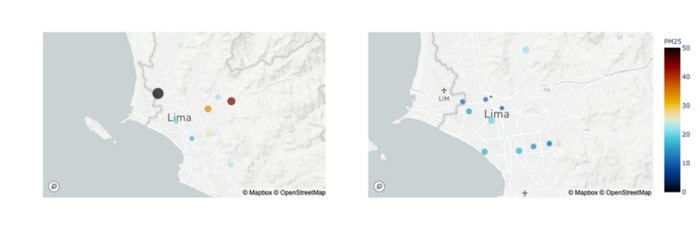
\includegraphics[width=.8\textwidth]{limamap.png}
    \caption{Ground-level air quality comparison in Lima, Peru: PM2.5 levels before (left) and after COVID19 (right) lockdown. Sources: QAIRA (Unicef Venture Fund), PlumeLab, OpenAQ.}
    \label{fig:limamap}
\end{figure*}

\begin{figure}[t]
    \centering
    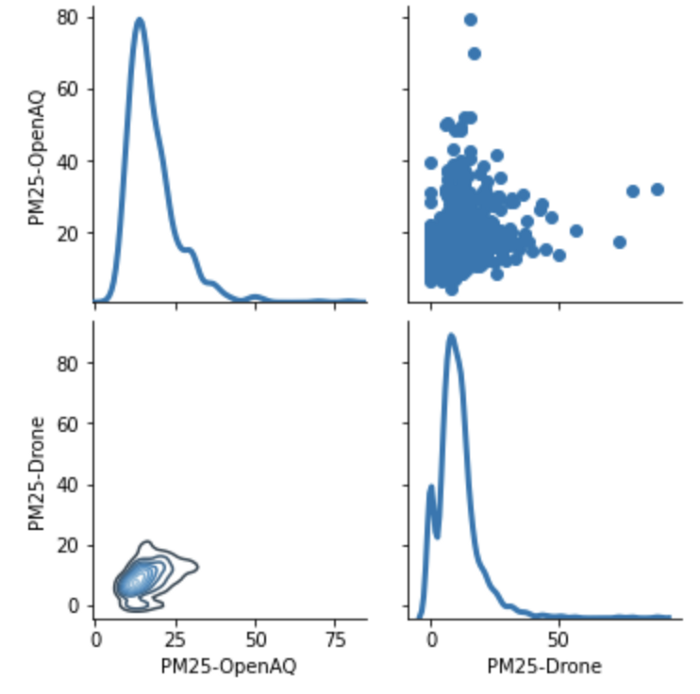
\includegraphics[width=.8\linewidth]{pmsummary.png}
    \caption{Comparison of PM2.5 readings from two different sources: Remote Sensing (OpenAQ) and ground-level (Drone).}
    \label{fig:summary}
\end{figure}

In this article, we have introduced the problem of developing a global-level machine learning model of accurately predicting air quality — especially in the wake of COVID19 imposed lockdowns —with multiple operational objectives. The next article shall incorporate the bi-level satellite data and features extracted from the secondary data sources in Table~\ref{tab:datatable} into an XGBoost to model PM2.5 globally. These secondary data sources include additional features such as population density and 2020 Covid-19 lockdown data that are known to significantly affect ground-level PM2.5 concentrations \cite{Hale}.
\section{Methodology}\label{sec:method}
\section{Results and discussion}\label{sec:res}

\bibliographystyle{apalike}
\bibliography{biblio}

\end{document}
